% *******************************************************************************
% * Copyright (c) 2007 by Elexis
% * All rights reserved. This document and the accompanying materials
% * are made available under the terms of the Eclipse Public License v1.0
% * which accompanies this distribution, and is available at
% * http://www.eclipse.org/legal/epl-v10.html
% *
% *  $Id: einfuehrung.tex 4904 2009-01-03 17:58:33Z rgw_ch $
%
%*******************************************************************************
% !Mode:: "TeX:UTF-8" (encoding info for WinEdt)

\section{Einleitung}
Views (Ansichten) sind die zentralen Anzeige- und Bedienungselemente in Elexis.
Eine View zeigt eine bestimmte Art von Daten in einer bestimmten Weise an und
kann definierte Bearbeitungen dieser Daten ermöglichen. Diese Views können Sie
je nach Bedürfnissen und Arbeitsgewohnheiten selbst zu sogenannten Perspektiven
zusammenstellen und abspeichern. Man auch an verschiedenen Arbeitsplätzen
verschiedene Perspektiven einrichten, da ja beispielsweise am Empfang, im Labor
und im Arztzimmer unterschiedliche Arbeiten im Vordergrund stehen.

Im Gegensatz zu anderen Praxisprogrammen wird bei Elexis die Benutzeroberfläche
also nicht vom Hersteller, sondern vom Anwender des Programms definiert.

In diesem Kapitel werden diejenigen Views beschrieben, die im Grundsystem von
Elexis eingeschlossen sind. Eine solche Aufzählung kann nie abschliessend sein,
da (von uns oder anderen) neu entwickelte Plugins jederzeit eigene Views
mitbringen können. Diese müssten dann in der Dokumentation des betreffenden
Plugins beschrieben sein.

\subsection{Öffnen und Schliessen einer View}
Alle im System vorhandenen Views (auch die, die von externen Plugins mitgebracht
werden) sind unter dem Menüpunkt \textsc{Fenster-Ansicht} erreichbar. In diesem
Menü finden sich manchmal einige Views, die für die aktuelle Perspektive
zusammengestellt wurden, sowie immer ein Menüpunkt \glqq Andere\ldots\grqq{}
resp. \glqq Other\ldots\grqq{}. Hier ist eine nach Themen gruppierte Liste aller
Views zu finden (s. Abb. \ref{fig:viewlist}).
%\usepackage{graphics} is needed for \includegraphics
\begin{figure}[htp]
\begin{center}
  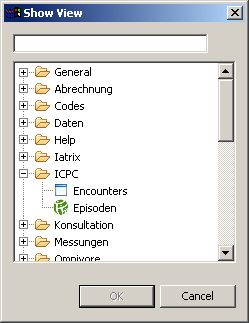
\includegraphics{images/showviewdialog}
  \caption{Liste aller Views}
  \label{fig:viewlist}
\end{center}
\end{figure}

Sie können entweder diese Liste durchblättern, oder Sie können den Namen der
gesuchten View im Textfeld oben eintippen. Sobald Sie anfangen zu tippen, wird
die Liste sofort auf die zu den getippten Buchstaben passenden Einträge
gefiltert.

Markieren Sie dann die gewünschte View und öffnen Sie sie entweder durch
Doppelklick oder Klick auf \glqq OK\grqq{}.

\par
Um eine View zu schliessen genügt es, auf das  X- Symbol im Karteireiter der
betreffenden View zu klicken.

\subsection{Öffnen und Speichern einer Perspektive}
\label{perspektiven} \index{Perspektive}
Eine Perspektive ist wie oben gesagt eine benannte Zusammenstellung von Views.
Elexis bringt einige vordefinierte Perspektiven mit, welche über die Startleiste
resp. die Toolbar aufgerufen werden können. (Vgl auch Abb. \ref{fig:toolbar}).

Eine Perspektive hat als \glqq Startperspektive\grqq{} eine spezielle Bedeutung:
Diese Perspektive wird immer automatisch nach dem Einloggen des entsprechenden
Anwenders auf dem betreffenden Arbeitsplatz eingestellt, sowie nach Klick auf das
'Home'-Symbol (der Button ganz links auf der Toolbar). Alle anderen (beliebig
viele) Perspektiven können unter einem frei wählbaren Namen abgespeichert und
wieder aufgerufen werden. Perspektiven sind Arbeitsplatz-Spezifisch (Eine auf
einem Arbeitsplatz eingestellte Perspektive steht also nicht automatisch auf
anderen Arbeitsplätzen zur Verfügung)\footnote{Dies muss so sein, da ja auch
nicht auf allen Arbeitsplätzen dieselben Plugins zur Verfügung stehen müssen -
vielleicht muss Ihr Buchhaltungs-Plugin nicht unbedingt auch auf dem Labor-PC
aktiv sein.}.

\begin{itemize}
\index{Perspektive!Startperspektive}
\item Um die aktuell eingestellte View-Anordnung als Startperspektive zu
speichern,
wählen Sie den Menüpunkt \textsc{Fenster -- Perspektive -- als Startperspektive
speichern}.

\item Um die aktuelle Perspektive neu (z.B. mit veränderter Viewanordnung oder
-Grösse) zu speichern, wählen Sie das Menü \textsc{Fenster -- Perspektive --
Speichere Perspektive}.

\item Um die aktuelle View-Anordnung unter einem eigenen Perspektivennamen
zu speichern, wählen Sie das  Menü \textsc{Fenster -- Perspektive -- Speichere Perspektive als\ldots}

\item Um die aktuelle Perspektive wiederherzustellen (falls Ihnen die gemachten
Ver\-än\-de\-run\-gen nicht zusagen, oder falls Sie versehentlich Views geschlossen
haben), wählen Sie \textsc{Fenster -- Perspektive -- Wiederherstellen}

\item Um zur Startperspektive zurückzukehren, klicken Sie auf das Haus-Symbol
ganz links in der Toolbar
\item Um eine früher gespeicherte Perspektive aufzurufen, wählen Sie
\textsc{Fenster -- Perspektive -- Andere} und wählen die gewünschte Perspektive
aus der Liste aus.

\end{itemize}
